\chapter{Indoor spatio-temporal movement patterns}
\section{Introduction}
As described in the firs part of this report, Wi-Fi tracking data can be used to
identify movement between buildings. Given that indoor areas are usually better
covered with Wi-Fi access points than outdoor areas, it is natural to also look
at movement inside buildings. The following section describes our method of
identifying and visualizing indoor movement in the Faculty of Architecture of TU
Delft.

The process of indoor movement analysis is conducted along the steps below,
thus the section also follows this structure:

\begin{enumerate}
    \item Delineate building parts based on the layout of access points
and the division of the building (e.g. department, canteen, building wing), and
group the access point into building parts.
    \item Identify movements in the data between building parts.
    \item Create a route network that connects the building parts and
    is constrained on the corridors of the building.
    \item Assign the movements to the route network.
    \item Visualize the movement along the indoor network.
\end{enumerate}

\section{Theory / methods}
After identifying movement between different buildings, the next level is to do
so between different parts inside a building. These parts represent
functional or spatial divisions inside a building, e.g. departments, community
areas, building wings and are referred to as \textit{building part}.

A prerequisite of the method is to know the at least room level location of the
access points in the respective building. At the time when the project
was carried out, the detailed access point locations were availably only for the
Faculty of Architecture. Thus the focus on this particular building.

As opposed to outdoor pedestrian movement which is not necessarily constrained
on a fixed network, indoor movement is constrained by the layout of the
respective building. The building parts of the Faculty of Architecture can be
represented by its underlying graph, having the building parts as nodes and the
corridors as edges \autoref{figure:bk_graph}. Then indoor movement is
necessarily constrained on this underlying graph.

\begin{figure}[H]
\centering
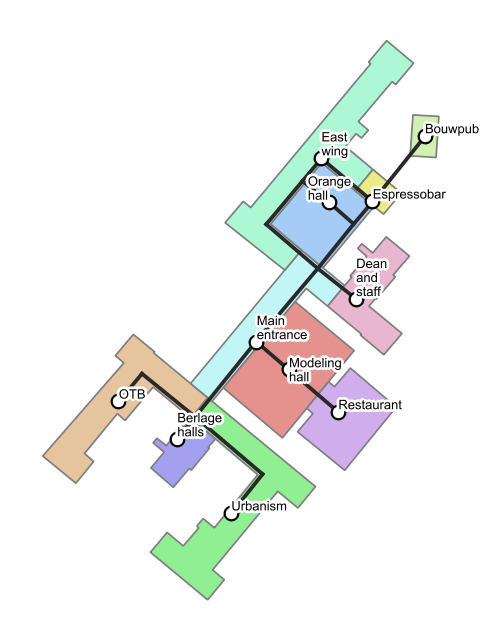
\includegraphics[scale=0.5]{bk_BG_bparts.png}
\captionsetup{justification=centering}
\caption{Building parts on the ground floor of the Faculty of Architecture and
its underlying graph.}
\label{figure:bk_graph}
\end{figure}

The Wi-Fi system of the TU Delft campus has a five minute scan interval, which
is too coarse to catch detailed movement indoor. As five minutes is
sufficient to reach any two locations in the building taking any route.
Therefore not the movement trajectory itself is identified from the data, but
the fact of relocation from origin to destination. Then the path of the movement
can also be identified by analysing the layout of the building. For example if a
person stayed at the Restaurant, then soon after he stayed at the Orange hall,
he necessarily had to traverse the corridors in-between these two locations. Our
method is based on this assumption.

Due to the building layout, in most of the cases there is only one possible
direct route between two building parts. However, in case of multiple route
options, the exact route of a movement is assumed to be the shortest route 
between origin and
destination.

\section{Implementation}
The identification and visualizatio of indoor movement ins a procedoure that
requires various tools and steps. While some steps can be automated, others need
to be done manually. The detailed description of these steps follows.

\subsection{Delineation of building parts}
There are two factors that define what is considered a building part, the layout
of the builidn and the layout of hte access points. The layout of the
builidng defines the functional divisions, e.g. departements or common areas.
Additionally, it is necessary to have at least one access point in each of these
divisions, or preferably more access points equally distributed in the division.
Considering the signal range of an access point, it is not desirable to have
access points close to the boarder of two neighbouring divisions, as in that
case the user could be falsly located in the neighbour division if he is picked
up by the respective access point. The combination of a functional division and
the access points within define a building part.

In case of the Faculty of Architecture \autoref{figure:BK_sketch} displays the
provided access point map and the manually overlaid functional divisions, thus
defining the building parts.
% TODO: put the complete list of building parts in the appendix and reference it
% here

\begin{figure}[H]
\centering
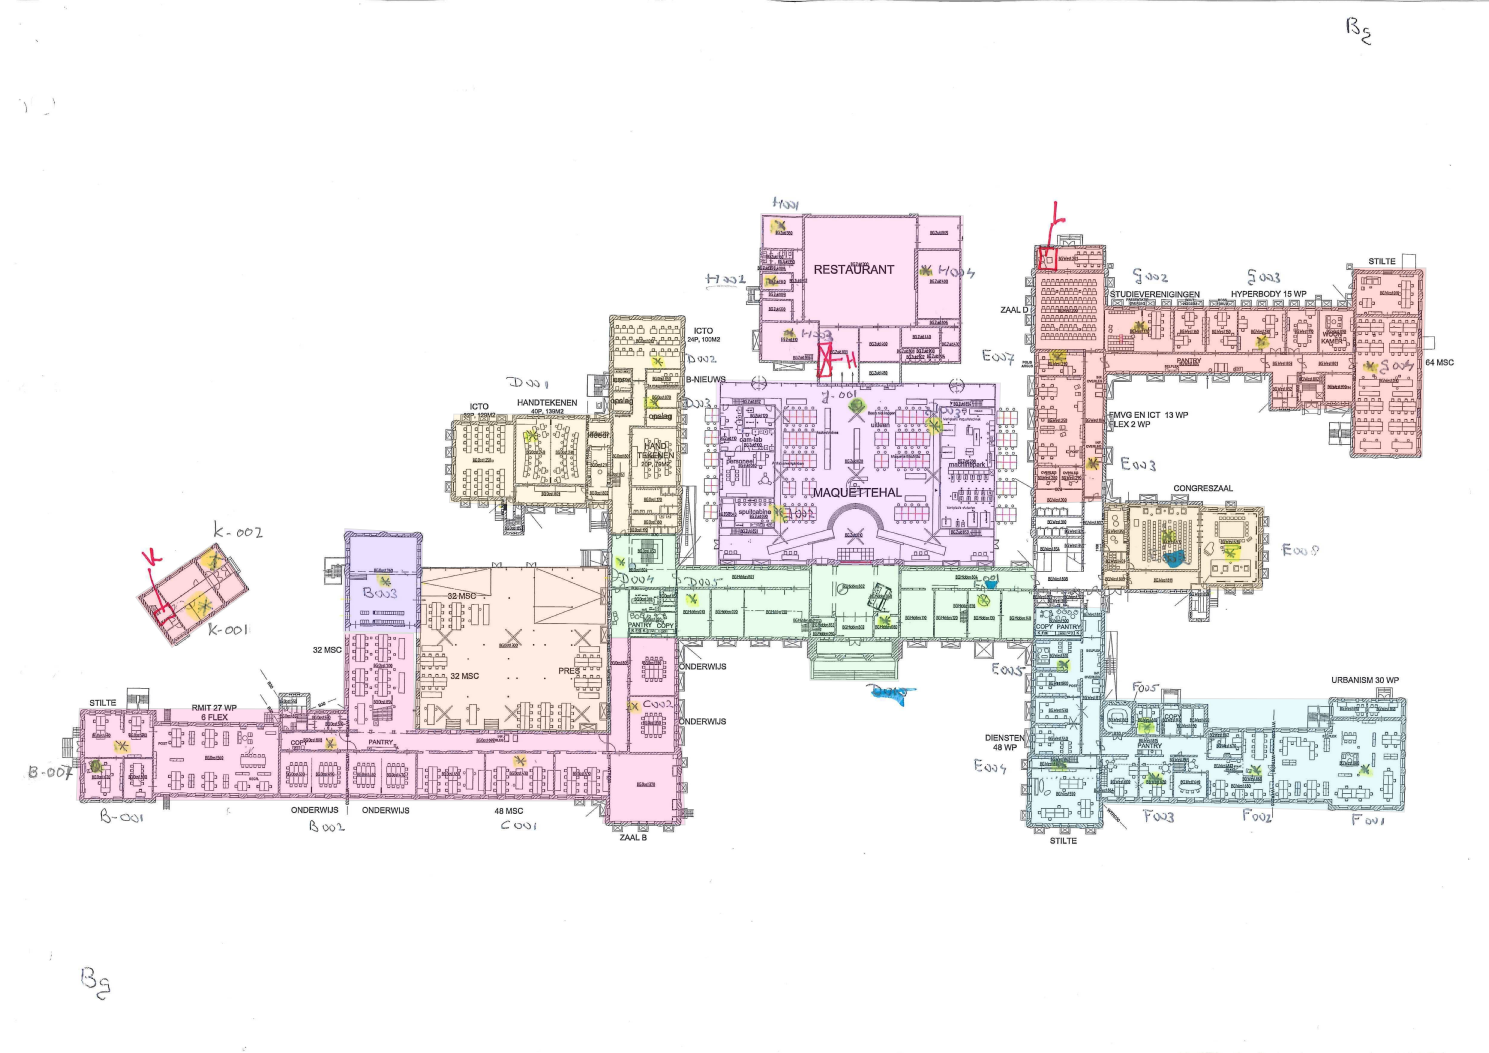
\includegraphics[scale=0.2]{bk_BG_sketch.png}
\captionsetup{justification=centering}
\caption{Access point map where yellow dots mark the access points, and
the functional divisions (colored areas) on the ground floor at the Faculty of
Architecture.}
\label{figure:BK_sketch}
\end{figure}

\subsection{Movement between building parts}

XANDER? or MARTIJN?

described the `movements table here`

\subsection{Indoor route network}
The route network of the Faculty of Architecture where nodes represent building
parts and edges represent corridors was drawn manually in \textit{QGIS},
following the floorplan of the building. However, the resulting \textit{sphagetti network}
does not contain the toplogical relations that are required to calculate
a shortest route. Therefore the topological relationships were created with the
PostGIS extension \textit{pgRouting}. Using a databased-based solution for
storing the data, creating toplogy and calculate shortest routes allowed us to
easily match the movements, which were calculated in the database, to the route
network.

\subsection{Mapping traffic to the route network}
In the \textit{movements table} every record represent a single move of a person
from origin to destination. In order to display these movements, identical moves
that have the same origin-destination pair are aggregated, resulting in a table
of unique origin-destination pairs with the amount of related moves
\autoref{table:moves}.

\begin{table}[H]
\centering
\caption{Aggregated moves between building parts}
\label{table:moves}
\begin{tabular}{@{}lll@{}}
\toprule
Origin        & Destination & Count \\ \midrule
OTB           & Restaurant  & 126   \\
Main entrance & Espressobar & 543   \\ \bottomrule
\end{tabular}
\end{table}

Then the shortest route between each origin-destination pair is calculated and
the movement counts are added to each edge that is traversed in the network.
Thus if the shortest route of two distinct movements share edges, the movement
count is summed up on the common edges, resulting in the traffic load of a given
edge \autoref{table:traffic}.

\begin{table}[H]
\centering
\caption{Traffic load on the indoor route network}
\label{table:traffic}
\begin{tabular}{@{}lll@{}}
\toprule
Edge ID & Traffic & Line width \\ \midrule
45      & 6151    & 1.10       \\
46      & 1994    & 0.64       \\ \bottomrule
\end{tabular}
\end{table}

% TODO: if we include code in the appendix, reference the function here

\subsection{Visualization of the movement}
The visualization method, as well as the route network, is two-dimensional.
However, three-dimensionality is imitated by using an \textit{exploded view}
common in architectural visualizations, that shifts overlapping elements (e.g.
floors) by a certain angle.

In this graphic the \textit{nodes} that represent the building parts are the approximate centroids of the polygonal area of the buildingpart. The nodes were manually adjusted
to better match the route network.

The route network is represented with
straigth lines, where the \textit{line width} is proportional to the traffic
load of a given edge. However, line widths cannot be compared across graphics, as in order
to facilitate consistent scale the line width variable is normalized to
the range of 0.5-5 units, regardless of traffic load. The range of 0.5-5 units
is choosen to provide a visually appealing and clear graphic. \textit{Colors}
mark the four separate floors and the staircases (grey) in the building.

\section{Results}

XANDER? or MARTIJN?
